\section{Cascade Bandwidth Design}
\begin{center}\begin{tabular}{llll}\ParamHeader
$\omega_i$ & Current target & $31415.93$ rad/s & Retained nominal target\\
$\omega_v$ & Load-speed target & $3141.59$ rad/s & Retained nominal target\\
$K_x$ & Position gain & $6.2832$ s$^{-1}$ & User setting\\
$B_l$ & Load-side damping & $N^2 B_m+B_g$ & Linear viscous model\\
\bottomrule\end{tabular}\end{center}
\[
P_i=\frac1{L_as+R},\quad C_i=\frac{\omega_i(L_as+R)}s,
\quad T_i=\frac{\omega_i}{s+\omega_i}
\]
\[
P_v=\frac{N}{Js+B_l},\quad
C_v=\frac{\omega_v(Js+B_l)}{Ns}
\]
\[
K_{p,v}=\frac{J\omega_v}{N},\quad
K_{i,v}=\frac{B_l\omega_v}{N},\quad
\frac{K_{i,v}}{K_{p,v}}=\frac{B_l}{J}
\]
\[
L_v^{ideal}=\frac{\omega_v}s,\quad
L_v=C_vT_iP_v,\quad T_v=\frac{L_v}{1+L_v},
\quad L_x=\frac{K_xT_v}{s},\quad T_x=\frac{L_x}{1+L_x}
\]
\textbf{Bode:} Open-loop 0 dB crossover versus closed-loop $-3$ dB bandwidth.
Position P control does not cancel a pole.
\textbf{Limits:} Nominal LTI model; gravity, saturation, sampling and residual back-EMF coupling excluded.
Current and speed targets require actuator feasibility assessment.
\IfFileExists{figures/cascade_bode.png}{\begin{center}
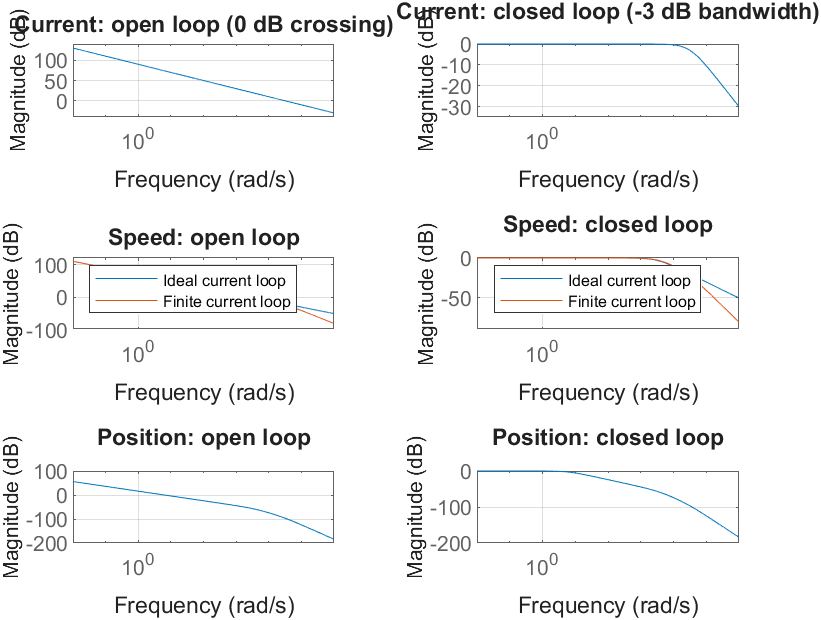
\includegraphics[width=\linewidth]{figures/cascade_bode.png}
\end{center}}{}

\subsection*{Verified Friction Path}
\[
\tau_{m,net}=\tau_m-B_m\omega_m,\quad
\omega_m=N\omega_l
\]
\[
N\tau_{m,net}=N\tau_m-N^2B_m\omega_l,
\qquad B_l=N^2B_m+B_g
\]
\textbf{Implementation:} Friction is already transformed by the signal path.
No additional $N^2$ gain is added to the friction block.
Speed PI assumes load-speed feedback.
